\documentclass[12pt, a4paper]{article}
\usepackage{enumitem}
\usepackage{float}
\usepackage[left=2cm, right=2cm, top=2cm, bottom=2cm]{geometry}
\usepackage{graphicx}
\usepackage[colorlinks, urlcolor=blue]{hyperref}
\usepackage[table]{xcolor}
\usepackage{xeCJK}

\renewcommand\arraystretch{1.1}
\setCJKmainfont[AutoFakeBold=1.5]{新細明體}

\title{
  Network Administration/System Administration\\
  (NTU CSIE, Spring 2024)\\
  Homework \#4
}
\author{\Large B12902110 呂承諺}

\begin{document}
  \maketitle
  \section*{Chapter1: 迷星叫}
  \begin{enumerate}
     \item\phantom{}\vspace{-\baselineskip}

     \begin{tabular}{|c|c|c|}
       \hline
       & 可通過的VLAN 數量 & 802.1Q 標記 \\\hline
       Access Port & 1 & No \\\hline
       Trunk Port & All in the allowlist & Yes, except for its native VLAN \\\hline
     \end{tabular}

     \item The trunk native VLAN is the VLAN that carries untagged traffic on a
     trunk port. On the transmitting side, packets with the same VLAN ID as the
     trunk native VLAN will be sent untagged. On the receiving side, untagged
     packets are assumed to be in the native VLAN.

     \item\phantom{}\vspace{-\baselineskip}

     \begin{tabular}{|c|c|c|c|c|c|c|}
       \hline
       \multicolumn{7}{|c|}{封包}\\\hline
       & \multicolumn{5}{c|}{802.1Q VID 欄位} & \\\hline
       傳遞方向 & 線路1 & 線路2 & 線路3 & 線路4 & 線路5 & 能否抵達 \\\hline
       PC-01/VLAN 10 → PC-02 & 10 & 無 & \cellcolor{gray} & \cellcolor{gray} & \cellcolor{gray} & 可 \\\hline
       PC-01/VLAN 20 → PC-02 & 10 & X & \cellcolor{gray} & \cellcolor{gray} & \cellcolor{gray} & 否 \\\hline
       PC-01/VLAN 10 → PC-04 & 10 & \cellcolor{gray} & X & \cellcolor{gray} & X & 否\\\hline
       PC-01/VLAN 20 → PC-04 & 20 & \cellcolor{gray} & 20 & \cellcolor{gray} & 20 & 可\\\hline
       PC-01/VLAN 10 → PC-03 & 10 & \cellcolor{gray} & \cellcolor{gray} & 10 & \cellcolor{gray} & 可 \\\hline
       PC-01/VLAN 20 → PC-03 & 20 & \cellcolor{gray} & \cellcolor{gray} & 20 & \cellcolor{gray} & 可 \\\hline
     \end{tabular}

     \item Suppose the packet has two VLAN tags, the first one with VLAN ID 10
     and the second one with VLAN ID 20. When Switch-01 forwards this packet to
     Switch-02 via link 3, it drops the first tag because VLAN 10 is the
     native VLAN for this trunk port. Now when Switch-02 receives the frame, it
     sees the tag with VLAN ID 20 and allows it to flow on link 5, eventually
     reaching PC-04.
  \end{enumerate}

  \paragraph{References}
  \begin{itemize}
    \item \href{https://www.cisco.com/en/US/docs/switches/datacenter/nexus5000/sw/configuration/nxos/Cisco_Nexus_5000_Series_NX-OS_Software_Configuration_Guide_chapter9.pdf}{Cisco\_Nexus\_5000\_Series\_NX-OS\_Software\_Configuration\_Guide\_chapter9.pdf}
    \item \href{https://community.cisco.com/t5/switching/vlan-tagging-on-access-port/td-p/4056567}{Solved: VLAN tagging on Access Port - Cisco Community}
    \item \href{https://networkengineering.stackexchange.com/questions/40483/arent-switch-access-ports-tagged}{vlan - Aren't Switch Access ports tagged? - Network Engineering Stack Exchange}
    \item \href{https://en.wikipedia.org/wiki/VLAN_hopping}{VLAN hopping - Wikipedia}
    \item \href{https://www.jannet.hk/virtual-lan-vlan-attack-zh-hant/}{VLAN Attack 虛擬區域網絡攻擊 - Jan Ho 的網絡世界}
  \end{itemize}
  \section*{Chapter2: 春日影}
  \subsection*{Part 1}
  \paragraph{Steps}
  \begin{enumerate}
    \item Open the backup configuration file, and we see\\
    \verb|username RiNG privilege 15 password 7 0813435D0C150C16|.
    \item According to the web, type 7 encryption is already cracked. We use the
    \href{https://www.firewall.cx/cisco/cisco-routers/cisco-type7-password-crack.html}{Cisco Type 7 Password Decrypt / Decoder / Crack Tool}
    and obtain password \verb|Roselia|.
  \end{enumerate}

  \paragraph{References}
  \begin{itemize}
    \item \href{https://www.cisco.com/c/en/us/td/docs/switches/lan/catalyst2960/software/release/15-0_2_se/configuration/guide/scg2960/swauthen.html}{Catalyst 2960, 2960-S, 2960-C, and 2960-Plus Switches Software Configuration Guide, Cisco IOS Release 15.0(2)SE and Later - Configuring Switch-Based Authentication [Cisco Catalyst 2960 Series Switches] - Cisco}
    \item \href{https://www.intesys.com.tw/edcontent_d.php?lang=tw&tb=10&cid=18&id=105}{常見問題 | Intesys 捷赫國際}
    \item \href{https://www.firewall.cx/cisco/cisco-routers/cisco-type7-password-crack.html}{Cisco Type 7 Password Decrypt / Decoder / Crack Tool}
  \end{itemize}

  \subsection*{Part 2}
  \paragraph{Steps}
  \begin{enumerate}
    \item Run the following commands on RiNG-Core:
\begin{verbatim}
RiNG-Core(config)#no vlan 10

RiNG-Core(config)#vlan 20
RiNG-Core(config-vlan)#name VLAN-MyGO
RiNG-Core(config)#interface range Fa0/1-3
RiNG-Core(config-if-range)#switchport access vlan 20

RiNG-Core(config)#vlan 30
RiNG-Core(config-vlan)#name VLAN-AveMujica
RiNG-Core(config)#interface range Fa0/11-12
RiNG-Core(config-if-range)#switchport access vlan 30

RiNG-Core(config)#interface Po1
RiNG-Core(config-if)#switchport trunk allowed vlan 20,99
\end{verbatim}
    \item Run the following commands on RiNG-Edge:
\begin{verbatim}
RiNG-Edge(config)#no vlan 10
RiNG-Edge(config)#vlan 20
RiNG-Edge(config-vlan)#name VLAN-MyGO

RiNG-Edge(config)#interface range Fa0/21-22
RiNG-Edge(config-if-range)#switchport access vlan 20

RiNG-Edge(config)#interface Po1
RiNG-Edge(config-if)#switchport trunk allowed vlan 20,99
\end{verbatim}
  \end{enumerate}

  \subsection*{Part 3}
   Run the following commands on RiNG-Core:
  \begin{enumerate}[label=\alph*.]
    \item
\begin{verbatim}
RiNG-Core(config)#no username RiNG
RiNG-Core(config)#username RiNG privilege 15 secret 0 Afterglow
\end{verbatim}
    \textbf{Note:} \verb|service password-encryption| is already on.

    \item
\begin{verbatim}
RiNG-Core(config)#ip domain-name RiNG
RiNG-Core(config)#crypto key generate rsa
The name for the keys will be: RiNG-Core.RiNG
Choose the size of the key modulus in the range of 360 to 4096 for your
  General Purpose Keys. Choosing a key modulus greater than 512 may take
  a few minutes.

How many bits in the modulus [512]: 4096
% Generating 4096 bit RSA keys, keys will be non-exportable...[OK]
\end{verbatim}
    \textbf{Note:} SSH version 2 requires the RSA key size to be at least 768
    bits.
    \item
\begin{verbatim}
RiNG-Core(config)#line vty 0 4
RiNG-Core(config-line)#login local
RiNG-Core(config-line)#transport input ssh
\end{verbatim}
    \item
\begin{verbatim}
RiNG-Core(config)#line vty 5 15
RiNG-Core(config-line)#transport input none
\end{verbatim}
    \item
\begin{verbatim}
RiNG-Core(config)#ip ssh version 2
\end{verbatim}
  \end{enumerate}
  Repeat all commands on RiNG-Edge except for \textit{b. SSH key generation},
  because it already has a key.

  \paragraph{References}
  \begin{itemize}
   \item \href{https://www.cisco.com/c/en/us/td/docs/switches/lan/catalyst2960/software/release/15-0_2_se/configuration/guide/scg2960/swauthen.html}{Catalyst 2960, 2960-S, 2960-C, and 2960-Plus Switches Software Configuration Guide, Cisco IOS Release 15.0(2)SE and Later - Configuring Switch-Based Authentication [Cisco Catalyst 2960 Series Switches] - Cisco}
  \end{itemize}

  \pagebreak
  \section*{Chapter3: 無路矢}
  \begin{enumerate}
    \item\phantom{}\vspace{-\baselineskip}

    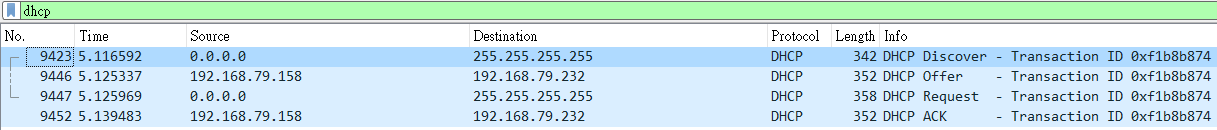
\includegraphics[width=0.9\textwidth]{wireshark_dhcp.png}

    \begin{itemize}
      \item \textbf{Discover:} The client sends a broadcast DHCPDISCOVER message
       to the current local network and hopes for response from a DHCP server.

      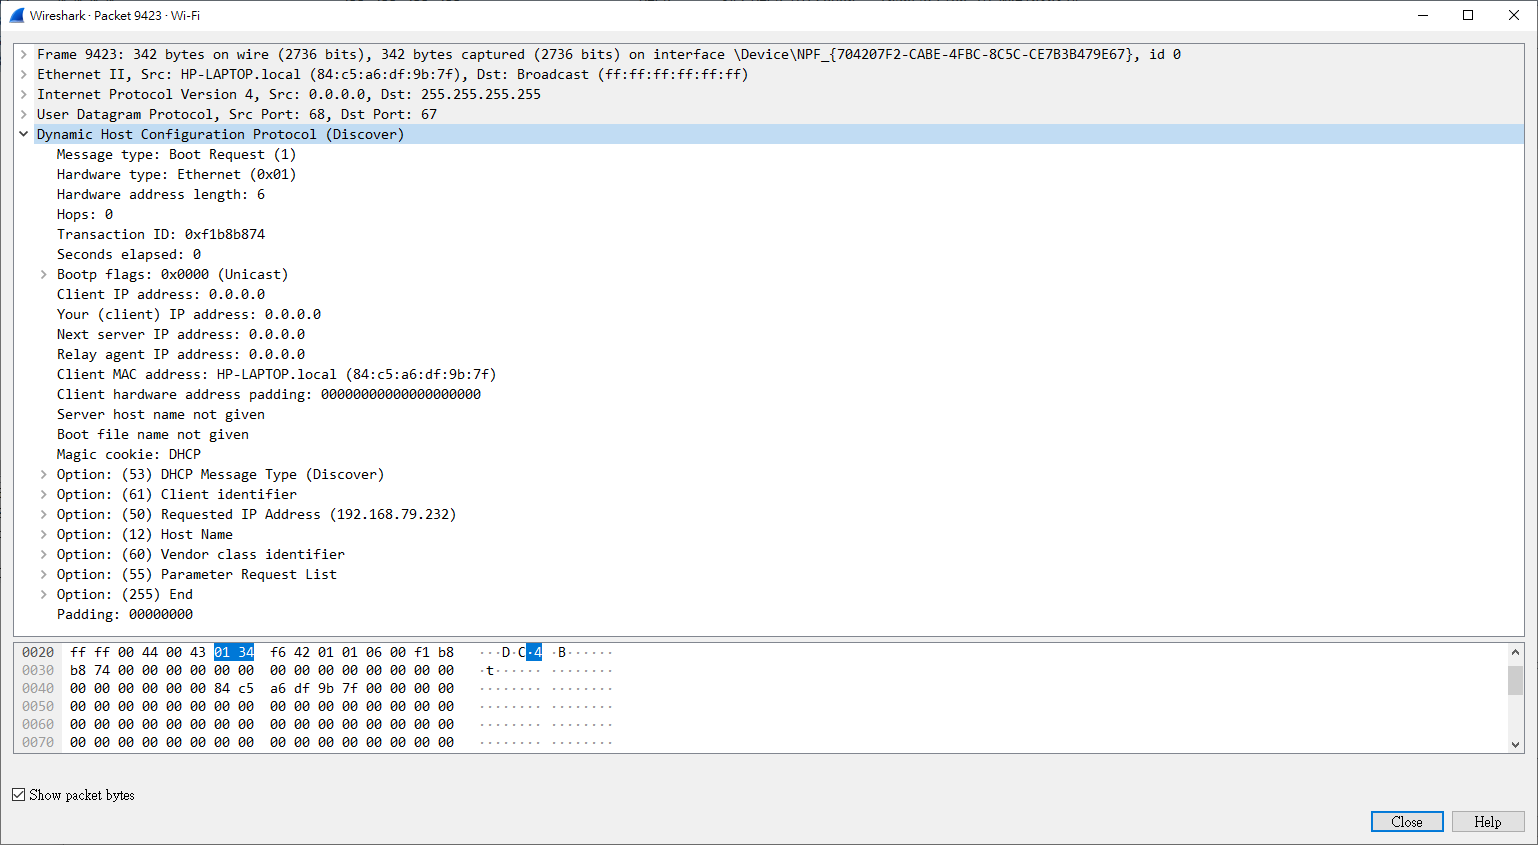
\includegraphics[width=0.8\textwidth]{wireshark_dhcp_discover.png}

      \item \textbf{Offer:} The DHCP server reserves an IP address for the
      client, and then sends a DHCPOFFER message to the client, offering a
      set of network configuration.

      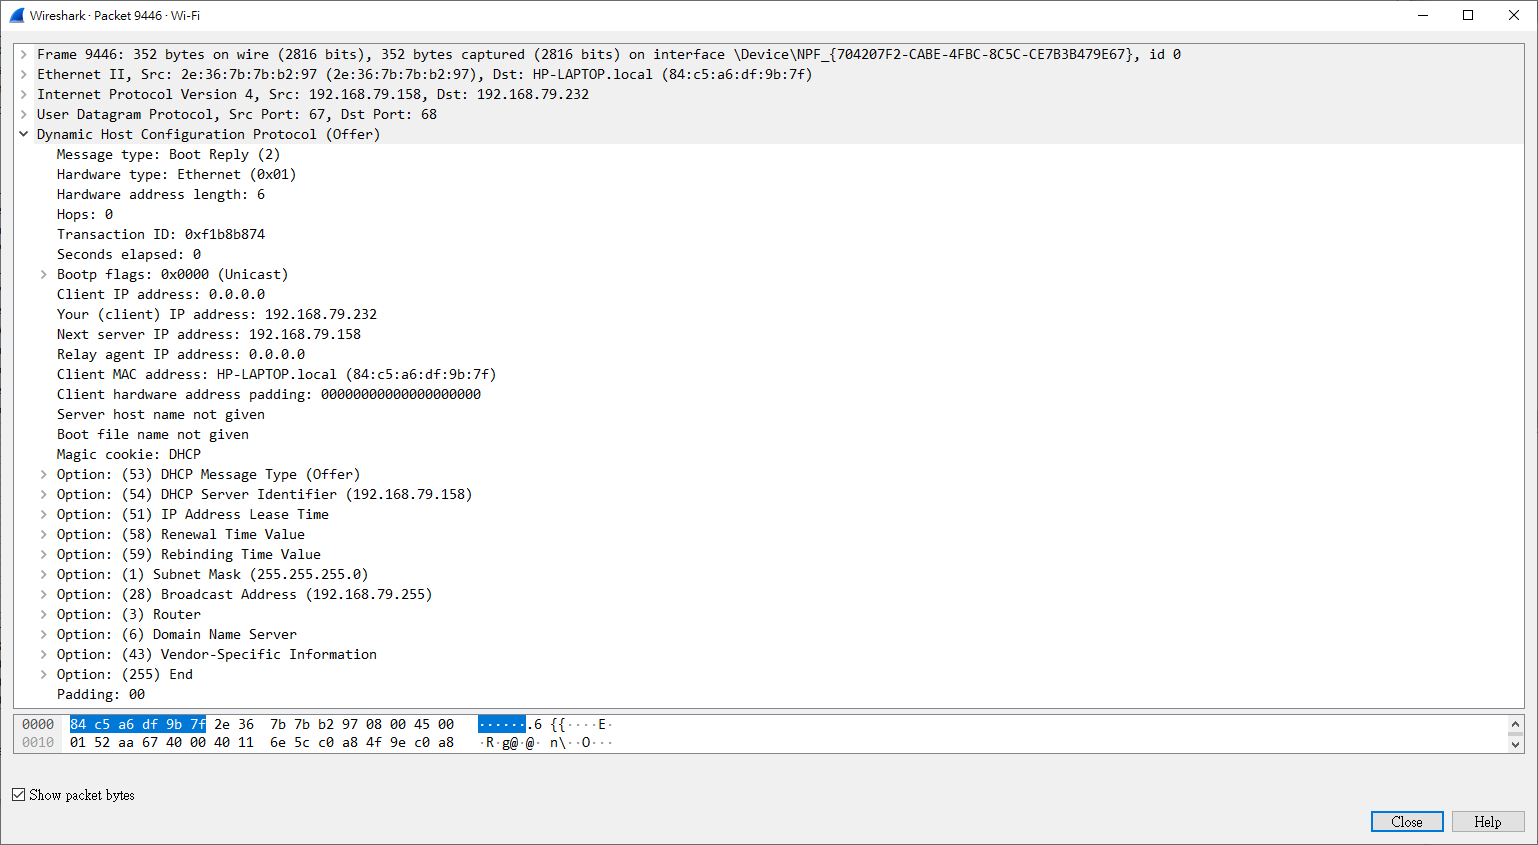
\includegraphics[width=0.8\textwidth]{wireshark_dhcp_offer.png}

      In this example, the server 192.168.79.158 give us an offer. The offered
      IP address is 192.168.79.232, subnet mask is 255.255.255.0, and
      default gateway is 192.168.79.158。

      \pagebreak
      \item \textbf{Request:} The client sends a broadcast DHCPREQUEST message
      to the server, requesting the IP address in the offer.

      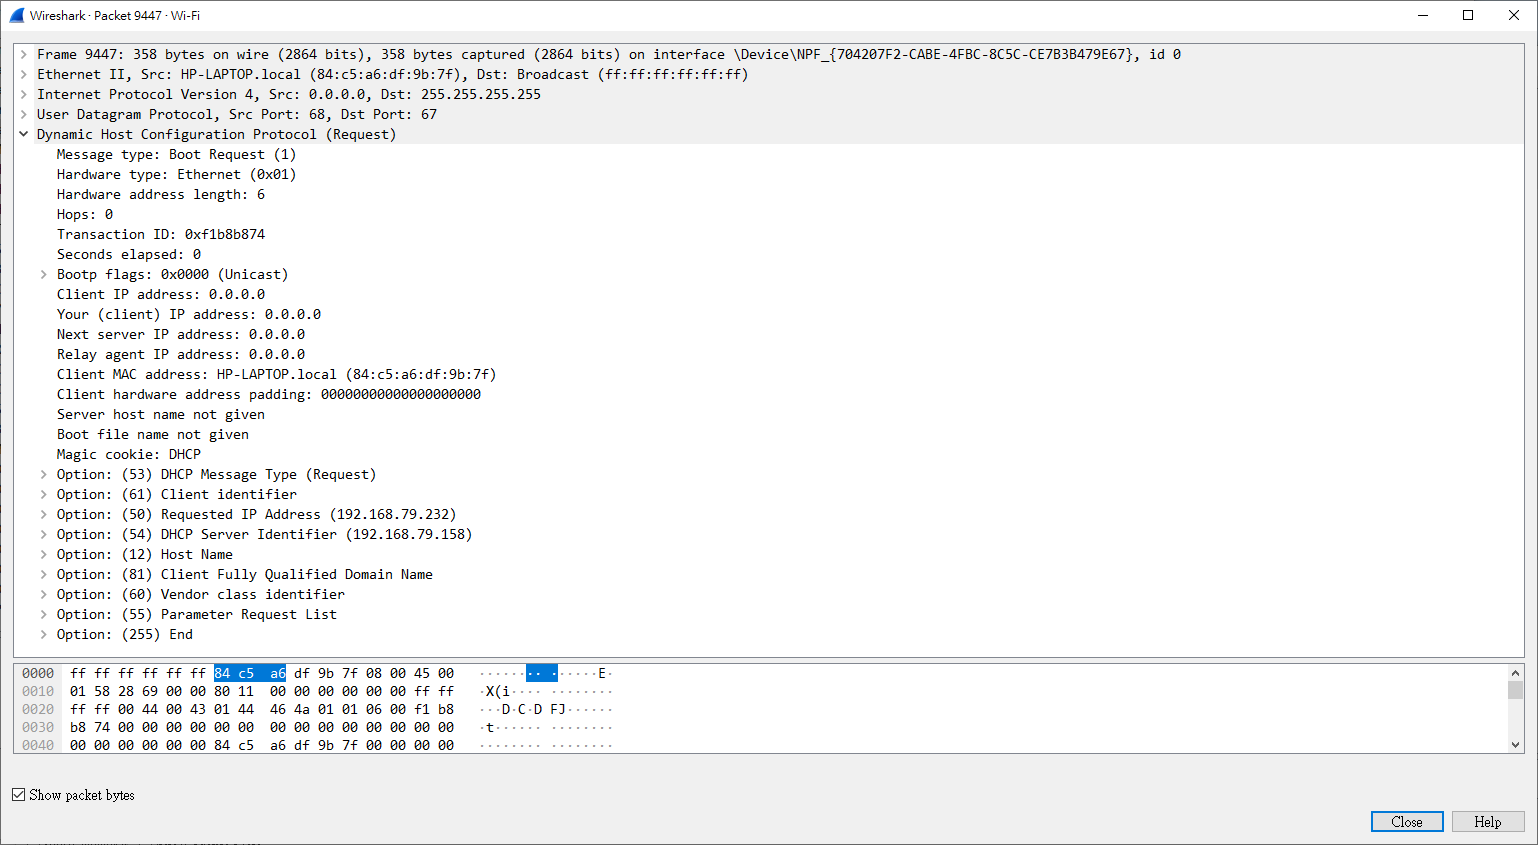
\includegraphics[width=0.8\textwidth]{wireshark_dhcp_request.png}

      In this example, that is 192.168.79.232。

      \item \textbf{Acknowledgement:} The server sends a DHCPACK message to
      the client and completes the setup.

      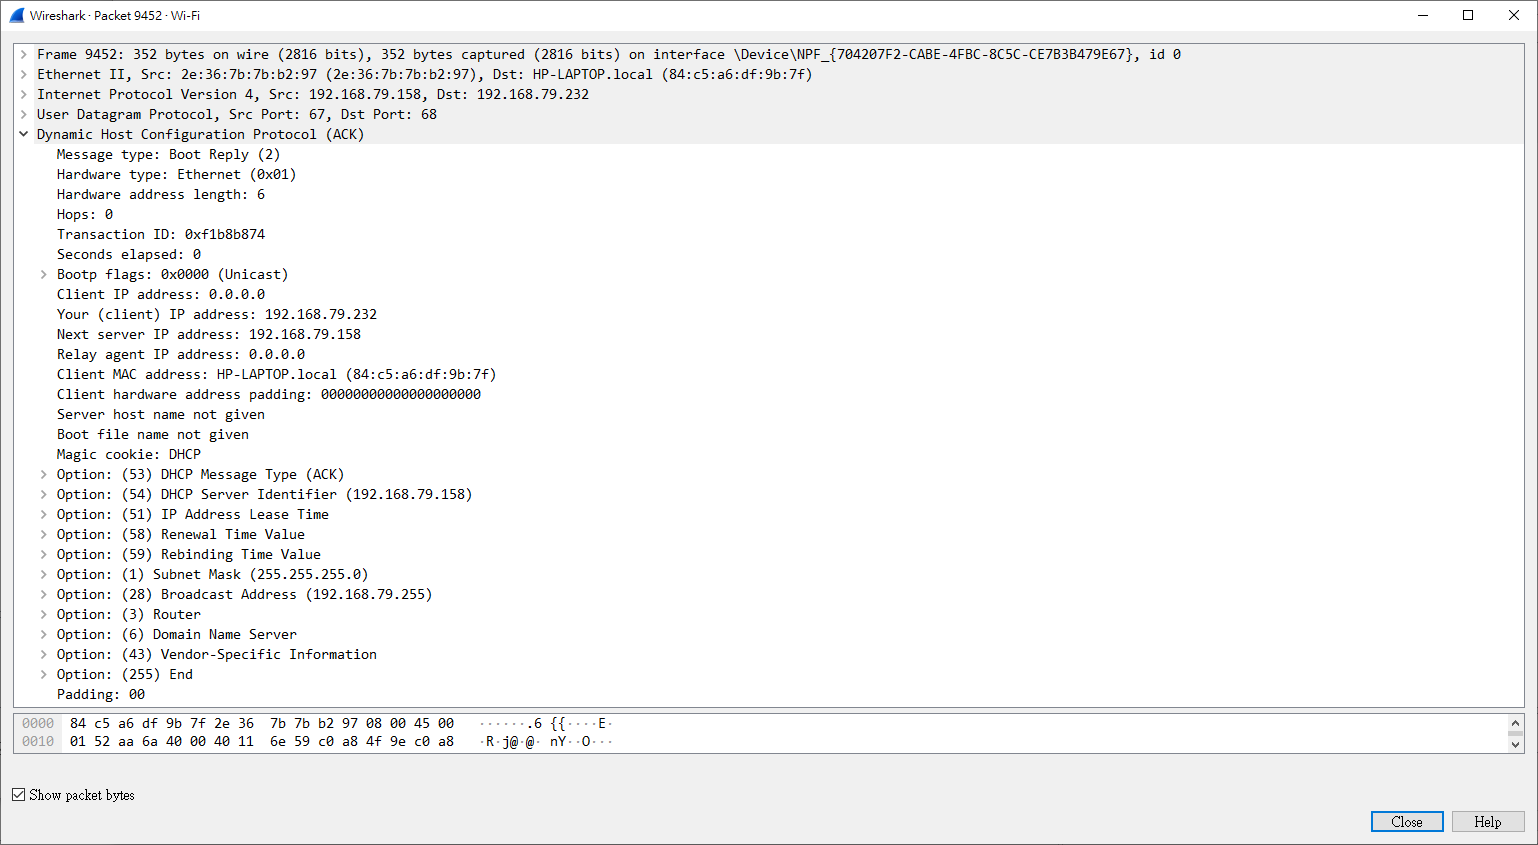
\includegraphics[width=0.8\textwidth]{wireshark_dhcp_ack.png}
    \end{itemize}

    \paragraph{References}
    \begin{itemize}
      \item \href{https://en.wikipedia.org/wiki/Dynamic_Host_Configuration_Protocol}{Dynamic Host Configuration Protocol - Wikipedia}
    \end{itemize}
    \item
    \begin{itemize}
      \item IP 0.0.0.0
      \begin{itemize}
        \item 涵義:目前所在的網路。
        \item 原因:用戶端還沒有IP位址。
      \end{itemize}
      \item IP 255.255.255.255
      \begin{itemize}
        \item 涵義:目前網路的廣播位址。路由器不會轉發送往255.255.255.255的封包到其他網路。
        \item 原因:連上網路的最初,用戶端不會知道DHCP伺服器的IP位址,因此廣播訊息給目前網路的所有裝置,期待有DHCP伺服器接收到。
      \end{itemize}
      \item MAC FF:FF:FF:FF:FF:FF
      \begin{itemize}
        \item 涵義:廣播MAC位址。送往這個位址的封包可以被所有LAN上的裝置接受到。
        \item 原因:連上網路的最初,用戶端不會知道DHCP伺服器的MAC位址,因此廣播訊息給目前網路的所有裝置,期待有DHCP伺服器接收到。
      \end{itemize}
    \end{itemize}

    \paragraph{References}
    \begin{itemize}
      \item \href{https://en.wikipedia.org/wiki/Reserved_IP_addresses}{Reserved IP addresses - Wikipedia}
      \item \href{https://en.wikipedia.org/wiki/Broadcast_address}{Broadcast address - Wikipedia}
    \end{itemize}

    \item Run the following commands to enable DHCP snooping:
\begin{verbatim}
RiNG-Core(config)#ip dhcp snooping
RiNG-Core(config)#ip dhcp snooping vlan 1
RiNG-Core(config)#interface Fa0/22
RiNG-Core(config-if)#ip dhcp snooping trust
\end{verbatim}
    \textbf{Note:} The default setting for an interface is untrusted.

    \paragraph{References}
    \begin{itemize}
      \item \href{https://en.wikipedia.org/wiki/DHCP_snooping}{DHCP snooping - Wikipedia}
      \item \href{https://www.cisco.com/c/en/us/td/docs/switches/lan/catalyst2960/software/release/15-0_2_se/configuration/guide/scg2960/swdhcp82.html}{Catalyst 2960, 2960-S, 2960-C, and 2960-Plus Switches Software Configuration Guide, Cisco IOS Release 15.0(2)SE and Later - Configuring DHCP Features and IP Source Guard [Cisco Catalyst 2960 Series Switches] - Cisco}
    \end{itemize}
  \end{enumerate}
\end{document}
